\chapter{Metodo - AMEGO} 
\emph{AMEGO}, acronimo di \emph{Active Memory of the EGOcentric video}, è concepito per trasformare un video egocentrico lungo e non strutturato in una memoria capace di descrivere in modo completo le interazioni del soggetto con oggetti e luoghi. Allo stesso tempo, può essere interrogato per recuperare i segmenti temporali in cui un oggetto è stato utilizzato, una location è stata visitata, o entrambe le condizioni si sono verificate contemporaneamente.

Un aspetto cruciale che distingue AMEGO da altri approcci riguarda la sua natura \emph{semantic-free}.  
Gli oggetti e le location non vengono legati a una tassonomia fissa di etichette o a un vocabolario prestabilito. Essi vengono invece rappresentati direttamente sulla base delle caratteristiche visive, consentendo così una distinzione più fine e dettagliata tra le diverse istanze. Questo approccio permette al sistema di adattarsi a contesti nuovi senza la necessità di ridefinire un insieme di categorie predefinite.

\section{Costruzione della memoria}
Dato un video egocentrico $\mathcal{V}$, esso viene scomposto in due elementi fondamentali:

\begin{itemize}
    \item \textbf{Hand-Object Interaction (HOI) tracklets}: ciascun HOI tracklet\footnote{\textbf{Tracklet}: sequenza di bounding box che identifica in modo coerente la traiettoria o l'interazione di un oggetto nel tempo.} descrive in maniera spaziotemporale un oggetto che interagisce in modo consistente con almeno una mano del soggetto. Ogni tracklet è caratterizzato da bounding boxes\footnote{\textbf{Bounding box}: regione rettangolare che delimita un oggetto in un singolo frame del video.} e dalle corrispondenti feature visive\footnote{\textbf{Feature visive}: rappresentazioni numeriche delle proprietà visive di un oggetto}.
    
    \item \textbf{Location segments}: ogni elemento corrisponde a un intervallo temporale in cui il soggetto si trova in un determinato luogo e vi svolge interazioni. L'interesse è focalizzato sulle cosiddette \emph{activity-centric-zones}, ossia i luoghi in cui avvengono le principali interazioni con gli oggetti.
\end{itemize}

Combinando gli \emph{HOI tracklets} con i \emph{Location segments} si ottiene una memoria strutturata in grado di eseguire i compiti discussi in precedenza.

La memoria viene definita come:
\[
\mathcal{E} = \{\mathcal{O}, \mathcal{L}\}
\]
dove:
\begin{itemize}
    \item $\mathcal{E}$: AMEGO
    \item $\mathcal{O}$: insieme di HOI tracklets
    \item $\mathcal{L}$: insieme dei Location Segments.
\end{itemize}

Questa memoria viene costruita \emph{online}, eliminando la necessità di riprocessare continuamente informazioni passate.

\subsection*{Object interaction tracklets}
Gli \emph{HOI tracklets}, indicati con $\mathcal{O}$ rappresentano sequenze di interazioni tra le mani del soggetto e gli oggetti presenti nel video. Formalmente, possiamo definire l'insieme degli HOI tracklets come:

\[
\mathcal{O} = \{ o_1, o_2, \dots, o_n \}
\]

dove ciascun tracklet $o_i \in \mathcal{O}$ è una tupla:

\[
o_i = (t_s, t_e, b_t, h, \text{id})
\]

con:
\begin{itemize}
    \item $t_s$: istante di inizio dell'interazione
    \item $t_e$: istante di fine dell'interazione
    \item $b_t$: sequenza di bounding box che raffigurano l'oggetto
    \item $h$: lato della mano che compie l'interazione (sinistra o destra)
    \item $\text{id}$: identificatore dell'istanza dell'oggetto associato al tracklet
\end{itemize}

La costruzione della memoria $\mathcal{O}$ avviene in maniera iterativa, processando il video frame per frame tramite una pipeline composta da tre fasi principali:

\begin{enumerate}
    \item \textbf{Initialization:} individuazione dei possibili nuovi HOI tracklets.
    \item \textbf{Updating:} aggiornamento dei tracklets attivi\footnote{\textbf{Tracklet attivi}: tracklets che stanno effettivamente registrando un'interazione in corso tra la mano del soggetto e l'oggetto}, corrispondenti alle interazioni in corso.
    \item \textbf{Assignment and storing:} i tracklets terminati \footnote{\textbf{Tracklet terminato}: l'azione per cui veniva considerato attivo è terminata} vengono archiviati nella memoria $\mathcal{E}$ e viene assegnata loro l'istanza oggetto corrispondente.
\end{enumerate}


\subsubsection*{Inizialization}
La prima fase consiste nell'individuazione dei nuovi \emph{HOI tracklets}. Per questo utilizziamo un detector di \emph{hand-object-interaction} \emph{class-agnostic}\footnote{\textbf{class-agnostic detector}: non fa distinzione tra classi predefinite di oggetti, ma identifica interazioni tra mani e oggetti basandosi su caratteristiche visive generiche} \cite{shan2020understandinghumanhandscontact}, che fornisce insiemi di bounding box attive per oggetti e mani, denotati rispettivamente come $\mathcal{B}_t^o$ e $\mathcal{B}_t^h$.

Un nuovo \emph{HOI tracklet} $o_i$ viene inizializzato per ciascuna nuova hand-object-interaction rilevata. Ogni tracklet è definito come una sequenza di almeno $s_o$ bounding box che mostrano un forte sovrapposizione spaziale all'interno di una finestra temporale di $w_s$ frame.

\begin{figure}[ht]
    \centering
    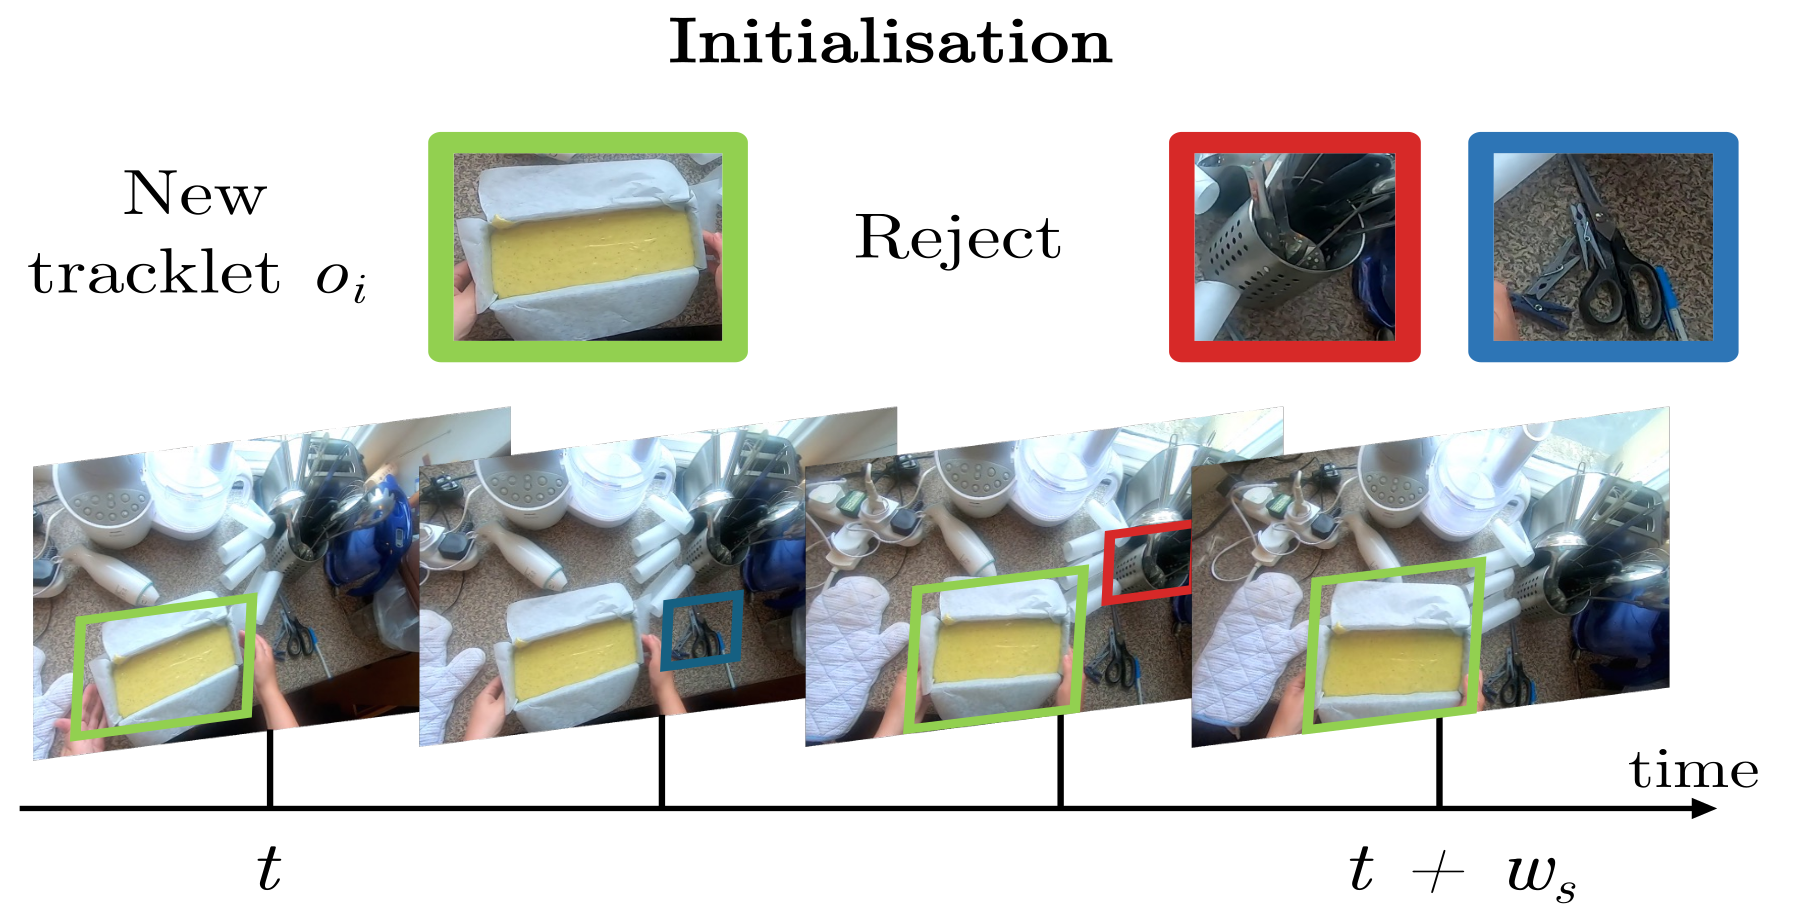
\includegraphics[width=0.8\textwidth]{Images/init.png}
    \caption{Fase di inizializzazione}
    \label{fig:init}
\end{figure}

Questo processo di filtraggio consente di ridurre il rumore generato dall'applicazione indipendente del rilevatore su ciascun frame. Considerando la durata naturale delle interazioni mano-oggetto, è possibile identificare in modo affidabile i nuovi tracklets attivi, garantendo coerenza spaziale e temporale nelle rilevazioni.  

Il tracklet $o_i$ viene ora considerato \emph{attivo} e aggiunto alla memoria $\mathcal{O}$.  

Per ciascun frame successivo, calcoliamo l'\emph{Intersection over Union (IoU)}\footnote{\textbf{Intersection over Union (IoU)}: misura di sovrapposizione tra due bounding box, calcolata come il rapporto tra l'area di intersezione e l'area di unione dei due rettangoli.} tra i bounding box degli oggetti che interagiscono con la stessa mano. I bounding box che superano una soglia $\theta$ vengono assegnati al tracklet $o_i$. Se non è possibile assegnare nuovi bounding box al tracklet, questo viene considerato \emph{terminato}.

\subsubsection*{Updating}

Questa fase mira a catturare l'intera durata dell'interazione e contemporaneamente a seguire tutte le occorrenze spaziali dell'oggetto.

Sebbene i rilevatori di HOI a livello di singolo frame siano sufficienti per identificare nuove interazioni, essi non sono in grado di estendere in modo affidabile i tracklets quando mani od oggetti escono dal campo visivo. Per questo motivo, viene utilizzato un \emph{single-object tracker (SOT)}\footnote{\textbf{Single-Object Tracker (SOT)}: permette di seguire un singolo oggetto nel tempo, stimando la posizione frame per frame anche in assenza di rilevazioni dirette.} \cite{tang2023egotrackslongtermegocentricvisual}.  

\begin{figure}[ht]
    \centering
    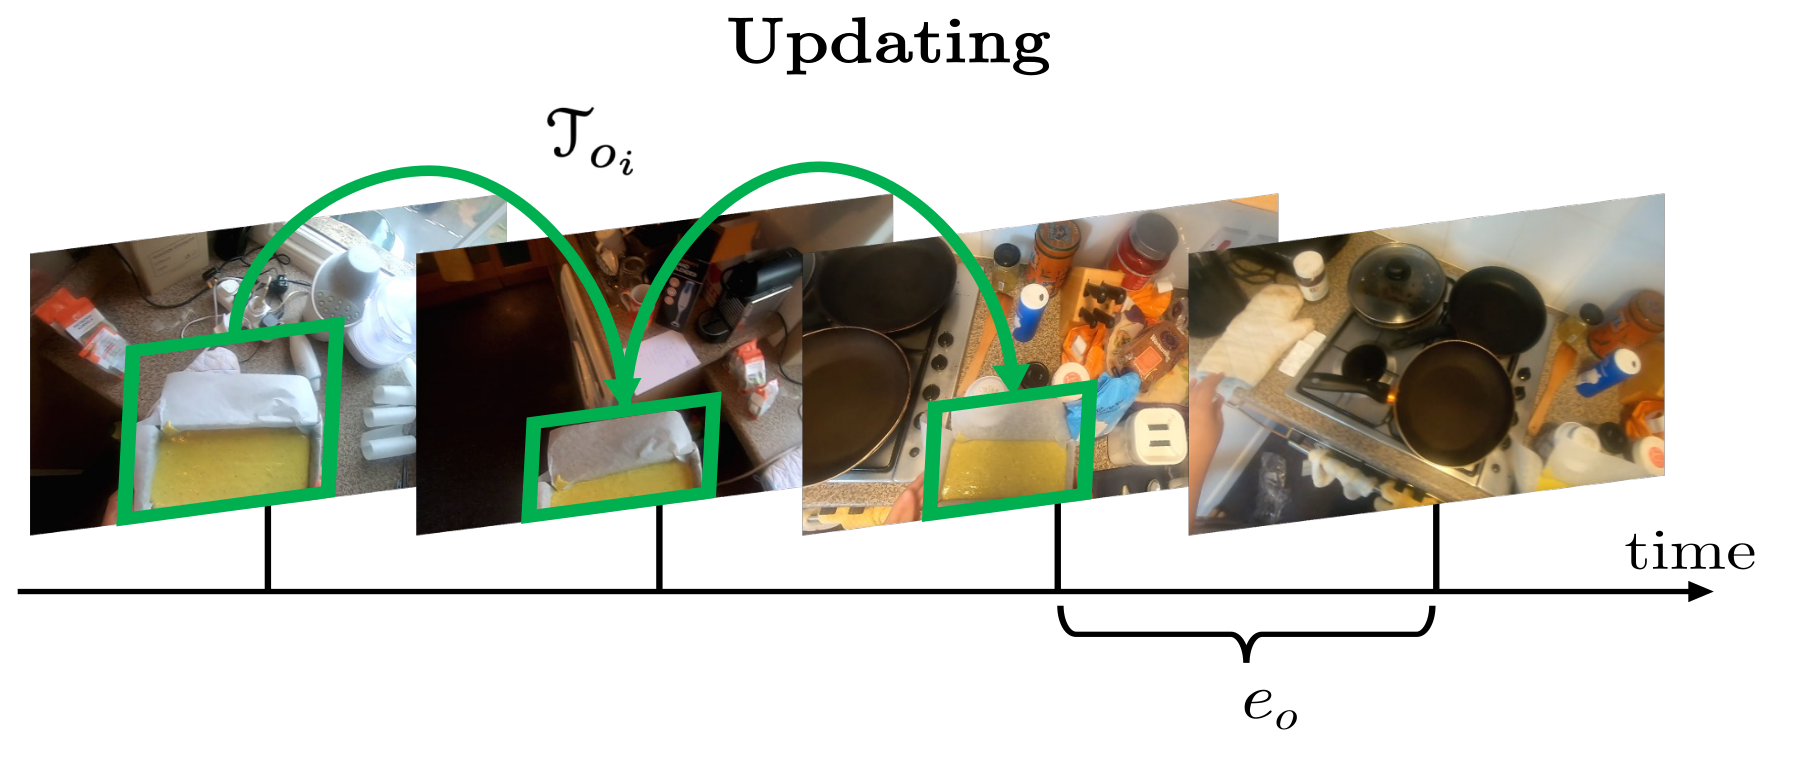
\includegraphics[width=0.8\textwidth]{Images/update.png}
    \caption{Fase di updating}
    \label{fig:update}
\end{figure}

Per ogni tracklet attivo $o_i$ viene inizializzato un SOT. Consideriamo il tracklet $o_i$ terminato se non sono presenti rilevazioni associate $\mathcal{B}^o$ per $e_o$ frame consecutivi, mentre la mano $h$ rimane visibile, in quanto quando la mano esce dal campo visivo è probabile che stia ancora tenendo l'oggetto.

L'output del SOT produce un track $\tau_{o_i}$ che segue la posizione dell'oggetto, ma non contiene informazioni sull'interazione stessa. A questo punto, $o_i$ combina le informazioni relative alla durata temporale (start ed end time) e ai bounding box spaziali dell'oggetto attivo, sfruttando sia la rilevazione HOI a livello di frame sia il tracciamento SOT.

\subsubsection*{Assignment and storing}

Come definito in precedenza, ogni HOI tracklet $o_i$ deve essere associato a una specifica istanza di oggetto. Per farlo, confrontiamo $o_i$ con le istanze già presenti nella memoria.  

In particolare, dato l'insieme di HOI tracklets già memorizzati al tempo $t$, denotato $\mathcal{O}_t$, e l'insieme dei tracciamenti SOT osservati nello stesso istante, $\tau_t$, verifichiamo se $o_i$ possa essere associato a un'istanza esistente o se sia necessario crearne una nuova. Per effettuare il confronto, calcoliamo prima le feature visive di $o_i$:

\[
f(o_i) = \frac{1}{|\mathcal{V}_{o_i}|} \sum_{k \in \mathcal{V}_{o_i}} \gamma(k, b_k^o)
\]

dove:
\begin{itemize}
    \item $\mathcal{V}_{o_i}$ è l'insieme dei frame associati a $o_i$,
    \item $b_k^o$ è il bounding box relativo al frame $k$,
    \item $\gamma$ visual-feature-extractor (nel caso di AMEGO: DINOv2 \cite{oquab2024dinov2learningrobustvisual}).
\end{itemize}

Per effettuare il \emph{matching}, utilizziamo un approccio di clustering online basato su $f(o_i)$. La similarità tra $o_i$ e una specifica istanza di oggetto $id_j$ viene calcolata come:

\[
s(o_i, id_j) = \frac{1}{|\mathcal{O}_t \in id_j|} \sum_{\mathcal{O}_t \in id_j} \langle f_{\mathcal{O}_t}, f_{o_i} \rangle
\]

dove $\langle \cdot, \cdot \rangle$ indica la \emph{cosine similarity} e $\mathcal{O}_t \in id_j$ è l'insieme dei tracklets associati all'istanza $id_j$.  

Assegniamo $o_i$ all'istanza $id_j^*$ che massimizza la similarità e che supera una soglia $\theta$ (diversa dalla soglia utilizzata per l'IoU). Se un tracker in $\tau_t$ si sovrappone significativamente con $o_i$ e la sua confidenza è maggiore della similarità massima, allora $o_i$ viene assegnato all'istanza del tracker. Altrimenti, viene assegnato a $id_j^*$. Qualora la similarità massima risultasse inferiore alla soglia, viene creata una nuova istanza per $o_i$.  

Al termine di questa fase, le feature $f(o_i)$ e l'istanza assegnata vengono associate al tracklet $o_i$ e memorizzate nella memoria $\mathcal{E}$

\begin{figure}[ht]
    \centering
    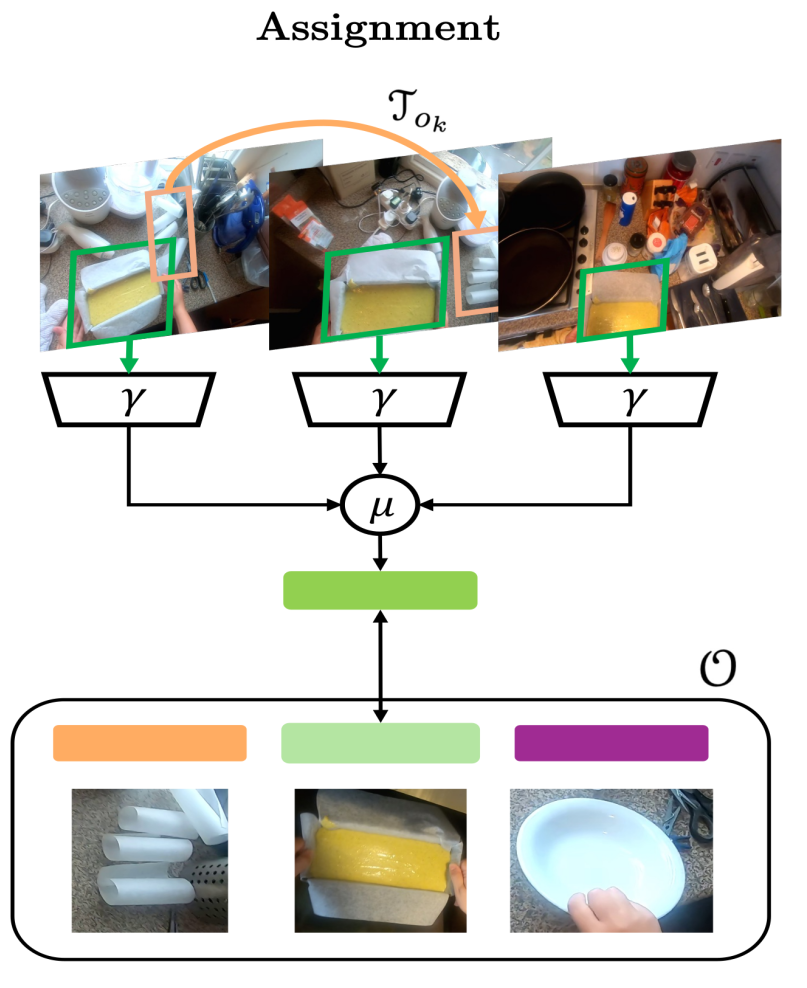
\includegraphics[width=0.4\textwidth]{Images/assign_store.png}
    \caption{Fase di assegnamento istanza}
    \label{fig:store}
\end{figure}

\subsection*{Location segments}
Definiamo l'insieme dei \emph{Location segments} $\mathcal{L}$ come gli intervalli temporali durante i quali il soggetto svolge interazioni in \emph{zone di attività principali}.

Poiché un soggetto può interagire con più oggetti simultaneamente ma può trovarsi in un solo punto alla volta, ogni segmento $l_i \in \mathcal{L}$ viene modellato come un intervallo temporale che corrisponde all'inizio e alla fine di un'interazione in quella specifica zona.  

Analogamente agli \emph{HOI tracklets}, l'insieme $\mathcal{L}$ viene costruito online.

Si seguendo due fasi principali: Temporal segmentation e Assignment and storing

\subsubsection*{Temporal segmentation}
Dati i frame $\mathcal{V}_t$ e le rilevazioni delle mani $B_t^h$, verifichiamo se la mano sta interagendo con un oggetto mentre si trova in una location. Per farlo, calcoliamo l'\emph{optical flow}\footnote{\textbf{Optical flow}: rappresenta il campo di movimento apparente dei pixel tra due frame consecutivi di un video, indicando la direzione e la velocità dello spostamento}tra $\mathcal{V}_{t-1}$ e $\mathcal{V}_t$ e controlliamo la presenza di mani assicurandoci che $|B_t^h|>0$.

Possiamo quindi determinare se il soggetto sta svolgendo un compito considerando le seguenti condizioni:
\begin{enumerate}
    \item l'\emph{optical flow} ha norma\footnote{\textbf{Norma}: grandezza che rappresenta l'intensità complessiva di un vettore, nel nostro caso l'optical flow} bassa;
    \item è rilevata almeno una mano.
\end{enumerate}
Questi criteri permettono di stabilire se il soggetto ha fatto una pausa (basso \emph{optical flow}) ed è attivamente coinvolto nella scena (mano rilevata).

Analogamente agli HOI, applichiamo un filtraggio temporale, per cui un \emph{Location segment} $l_j$ è considerato attivo solo se entrambe le condizioni sono verificate per un numero consecutivo di frame $s_l$. Il segmento $l_j$ viene terminato quando osserviamo un numero consecutivo di frame $e_l$ in cui la norma dell'\emph{optical flow} supera la soglia o non sono presenti mani rilevate.

\subsubsection*{Assignment and storing}
Come per gli HOI, dobbiamo assegnare un'istanza alle location $l_j$ definite temporaneamente. Agiamo analogamente, utilizzando però un \emph{visual-feature-extractor} differente, $\sigma$ (SWAG)\cite{singh2022revisitingweaklysupervisedpretraining}.

Una volta ottenute le visual-feature $g_{l_j}$, calcoliamo la similarità tra tutte le istanze di location già presenti e assegniamo a $l_j$ l'id che massimizza questa similarità, a condizione che superi una soglia prestabilita $\tau$. Se la soglia non viene superata, viene creata una nuova istanza.

\[
s(l_j, id_j) = \frac{1}{|\mathcal{L}_t \in id_j|} \sum_{\mathcal{L}_t \in id_j} \langle g_{\mathcal{L}_t}, g_{l_j} \rangle
\]

Al termine di queste fasi, assegniamo $g(l_j)$ e l'istanza correlata nella nostra memoria $\mathcal{E}$.

\section{Pseudocodici}

Di seguito vengono riportati i pseudocodici relativi alla costruzione della pipeline per la generazione degli elementi della memoria discussi nei paragrafi precedenti.
\subsection*{Object interactions}
\begin{algorithm}[H]
    \caption{Object interactions pipeline}
    \begin{algorithmic}[1]
    \State \textbf{Input:}
    \State \quad Frames $\{\mathcal{V}_t\}$
    \State \quad HOI detector $\mathcal{D}$
    \State \quad SOT tracker $\mathcal{J}$
    \State \quad Similarity threshold $\theta$
    \State \textbf{Output:}
    \State \quad Set of hand-object interaction tracklets $\mathcal{O}$
    \For{each frame $\mathcal{V}_t$}
        \State $\mathcal{B}_t^o, \mathcal{B}_t^h \gets \mathcal{D}(\mathcal{V}_t)$ (Detect hands and objects)
        \For{each detection $(b^o, b^h) \in (\mathcal{B}_t^o, \mathcal{B}_t^h)$}
            \If{new HOI\footnote{\textbf{hoi}: hand-object interaction} (i.e. $s_o$ detections in the last $w_s$ frames)}
                \State Create new tracklet $o_i$
                \State Start SOT $mathcal{J}_{o_i}$ for $o_i$
            \EndIf
        \EndFor
        \For{each \textbf{completed} tracklet $o_i$}
            \State Update the detections with $\mathcal{J}_{o_i}$
            \If{$\nexists b^o \in \mathcal{B}_t^o$ matching with $o_i$ in the last $e_o$ frames and $|\mathcal{B}_t^o|>0$}
                \State Mark $o_i$ as complete
            \EndIf
        \EndFor
    \EndFor
    \For{each completed tracklet $o_i$}
        \State Compute visual features $f(o_i)$
        \State Compute similarity $s(o_i, id_j)$ with existing instances in $\mathcal{O}$
        \If{maximum similarity $>\theta$}
            \State Assign $o_i$ to best matching instance $id_j$
        \Else
            \State Create new instance for $o_i$
        \EndIf
        \State Store $o_i$ in $\mathcal{O}$
    \EndFor
    \State \textbf{return} $\mathcal{O}$
    \end{algorithmic}
\end{algorithm}

\subsection*{Location segments}
\begin{algorithm}[H]
    \caption{Location Segment pipeline}
    \begin{algorithmic}[1]
    \State \textbf{Input:}
    \State \quad Frames $\{\mathcal{V}_t\}$
    \State \quad HOI detector $\mathcal{D}$
    \State \quad Similarity threshold $\tau$
    \State \textbf{Output:}
    \State \quad Set of location segments $\mathcal{L}$
    \For{each frame $\mathcal{V}_t$}
        \State $\mathcal{B}_t^o, \mathcal{B}_t^h \gets \mathcal{D}(\mathcal{V}_t)$ (Detect hands and objects)
        \State Compute optical flow OpticalFlow($\mathcal{V}_{t-1}, \mathcal{V}_t$)
        \If{location segment $l_j$ is active}
            \If{high $|\text{OpticalFlow}(\mathcal{V}_{t-1}, \mathcal{V}_t)|$ or $|\mathcal{B}_t^h| = 0$ for $e_l$ consecutive frames}
                \State Mark $l_j$ as complete
            \Else
                \State Continue $l_j$
            \EndIf
        \Else
            \If{low $|\text{OpticalFlow}(\mathcal{V}_{t-1}, \mathcal{V}_t)|$ and $|\mathcal{B}_t^h| > 0$ for $s_l$ consecutive frames}
                \State Subject is interacting, start active location segment $l_j$
            \EndIf
        \EndIf
    \EndFor
    \For{each completed segment $l_j$}
        \State Compute visual features $g(l_j)$
        \State Compute similarity $s(l_j, id_i)$ with existing instances in $\mathcal{L}$
        \If{maximum similarity $>\tau$}
            \State Assign $l_j$ to best matching instance $id_i$
        \Else
            \State Create new instance for $l_j$
        \EndIf
        \State Store $l_j$ in $\mathcal{L}$
    \EndFor
    \State \textbf{return} $\mathcal{L}$
    \end{algorithmic}
\end{algorithm}    


\section{AMB - Active Memories Benchmark}
Per studiare le interazioni dei vari elementi è stato introdotto un benchmark ad-hoc, l'\emph{Active Memories Benchmark} (AMB).

Il benchmark comprende 20.500 query che coprono diversi livelli di ragionamento. Le query sono formulate come domande a scelta multipla.

Ad esempio, alcune domande riguardano l'utilizzo di oggetti: ``Quale oggetto ho usato con [VQ]?'' dove [VQ] rappresenta un ritaglio visivo dell'oggetto; altre domande chiedono ``In quali location ho usato [VQ]?''

\begin{figure}[ht]
    \centering
    \includegraphics[width=0.8\textwidth]{Images/benchmark.png}
    \caption{Query del benchmark AMB}
    \label{fig:benchmark_queries}
\end{figure}

Come si nota, nelle domande non compaiono i nomi degli oggetti. Ogni visual query di un oggetto (VQ), risposta visiva dell'oggetto (VA), query sulla location (LQ) o risposta sulla location (LA) è parametrizzata tramite patch visive.

\subsection*{Tipologie di query}

Le query sono strutturate in tre macro aree:
\begin{itemize}
    \item \textbf{\textcolor{sqcolor}{Sequencing (SQ) [Q1-4]}}: valutano la capacità di discriminare l'ordine temporale degli eventi. Ad esempio, il modello deve ordinare le interazioni nel tempo e identificare quale oggetto è stato utilizzato prima o dopo un altro.
    
    \item \textbf{\textcolor{cocolor}{Concurrency (CO) [Q5-6]}}: valutano la capacità di catturare interazioni multiple simultanee. Ad esempio, verificare se diversi oggetti sono stati utilizzati insieme (oggetto-oggetto) o se un oggetto è stato usato in una specifica location (oggetto-location).
    
    \item \textbf{\textcolor{tgcolor}{Temporal Grounding (TG) [Q7-8]}}: valutano la capacità di recuperare tutti gli intervalli temporali in cui un oggetto o una location è stato coinvolto in interazioni.
\end{itemize}

\begin{table}[ht]
    \begin{center}
        \scriptsize % font più piccolo
        \setlength{\tabcolsep}{3pt} % riduce lo spazio tra colonne
        \renewcommand{\arraystretch}{1.2} % aumenta leggermente l'altezza delle righe
        \begin{tabular}{|p{1.8cm}|p{1cm}|p{7cm}|p{1cm}|p{1.5cm}|}
        \hline
        \textbf{Reasoning} & \textbf{Query} & \textbf{Template} & \textbf{Dim.} & \textbf{Answer} \\
        \hline
        \multirow{4}{*}{\textcolor[HTML]{789ECC}{SQ}} 
        & \textcolor[HTML]{789ECC}{Q1} & \raggedright What is the correct sequence of objects I have interacted with? & O & Obj. seqs \\
        \cline{2-5}
        & \textcolor[HTML]{789ECC}{Q2} & \raggedright What did I use with the left/right hand after [VQ]? & O & Obj. \\
        \cline{2-5}
        & \textcolor[HTML]{789ECC}{Q3} & \raggedright What did I use with the left/right hand before [VQ]? & O & Obj. \\
        \cline{2-5}
        & \textcolor[HTML]{789ECC}{Q4} & \raggedright Where did I take/leave [VQ]? & O, L & Loc. \\
        \hline
        \multirow{2}{*}{\textcolor[HTML]{C23A21}{CO}} 
        & \textcolor[HTML]{C23A21}{Q5} & \raggedright What did I use with [VQ]? & O & Obj. sets \\
        \cline{2-5}
        & \textcolor[HTML]{C23A21}{Q6} & \raggedright Where did I use [VQ]? & O, L & Loc. sets \\
        \hline
        \multirow{2}{*}{\textcolor[HTML]{02BF3D}{TG}} 
        & \textcolor[HTML]{02BF3D}{Q7} & \raggedright When did I use [VQ]? & O & Intervals \\
        \cline{2-5}
        & \textcolor[HTML]{02BF3D}{Q8} & \raggedright When did I visit [LQ]? & O, L & Intervals \\
        \hline
        \end{tabular}
        \caption{Tipologie di domande AMB con colonne colorate per tipo di Reasoning}
        \label{tab:amb_queries_colored}
    \end{center}
\end{table}  

\subsection*{Risposte alle Query}

Inizialmente, si recupera la rappresentazione più vicina dell'oggetto o della location della query, quindi vengono applicate euristiche specifiche per ciascuna domanda. Un esempio viene fornito al seguente link: \url{https://gabrielegoletto.github.io/AMEGO/#querying}.  
Di seguito vengono spiegati i dettagli teorici delle implementazioni.

\subsubsection*{Q1: Sequenze di oggetti}
Si confrontano tutti gli oggetti presenti nelle sequenze associate a ciascuna risposta, assegnando ogni patch d'immagine a un oggetto $q\_id$ tra quelli in $\mathcal{O}$. Successivamente, si seleziona la risposta con la sottosequenza comune più lunga calcolata tra la sequenza completa di $\mathcal{O}$ e ciascuna delle risposte.

\begin{figure}[H]
    \centering
    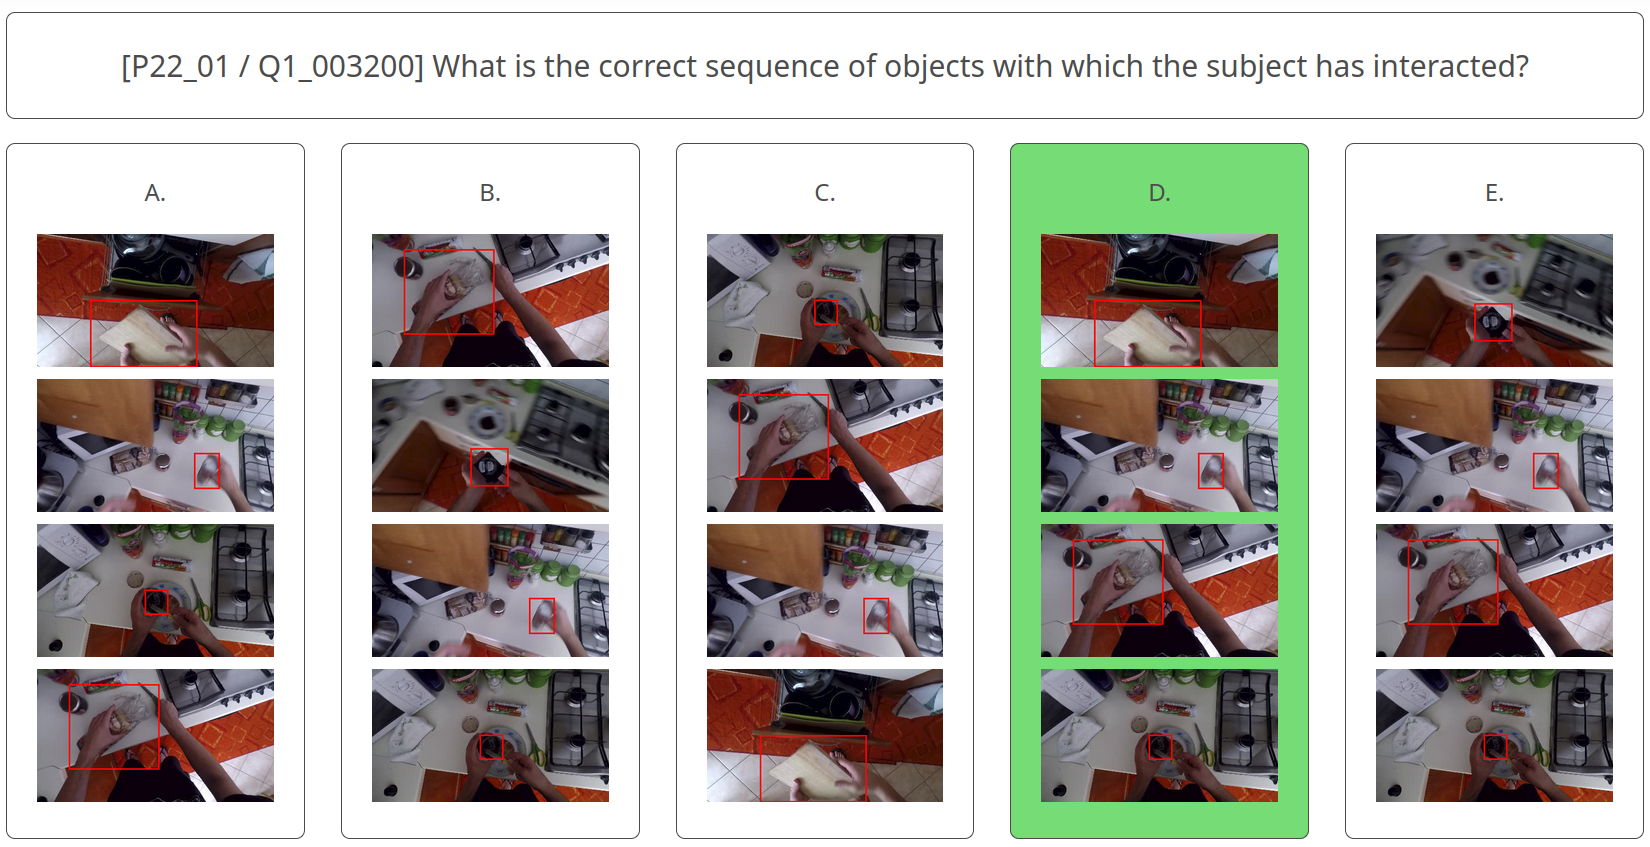
\includegraphics[width=0.9\textwidth]{Images/q1_res.png}
    \caption{Esempio di risposta a Q1.}
    \label{fig:q1_example}
\end{figure}

\subsubsection*{Q2-Q3: Oggetto prima o dopo la query}
Si identifica la traccia dell'oggetto della query in $\mathcal{O}$ basandosi su tre criteri:
\begin{itemize}
    \item vicinanza temporale a $t$;
    \item presenza del lato della mano indicato nella domanda;
    \item similarità minima di 0.6.
\end{itemize}
Una volta individuata la traccia corrispondente, per Q2 si estrae la parte successiva della traccia contenente la mano della query, mentre per Q3 si estrae la parte precedente, confrontandola con le risposte e selezionando quella con la similarità più alta.

\subsubsection*{Q4: Location iniziale/finale}
Si individua l'oggetto della query in $\mathcal{O}$ e il corrispondente $q\_id$. Usando questo ID, si identifica il primo o l'ultimo segmento di location in cui l'oggetto appare in $\mathcal{E}$ e si confrontano le location con le risposte. La risposta selezionata è quella con la similarità più alta.

\subsubsection*{Q5: Oggetti concorrenti}
Si confronta l'oggetto della query con le tracce in $\mathcal{O}$ per ottenere il $q\_id$. Allo stesso modo, si estraggono gli ID degli oggetti di ciascuna risposta. La risposta selezionata è quella con il maggior numero di oggetti che coesistono temporalmente con $q\_id$ (segmenti temporali sovrapposti) in $\mathcal{E}$.

\begin{figure}[H]
    \centering
    \includegraphics[width=0.9\textwidth]{Images/q5_res.png}
    \caption{Esempio di risposta a Q5.}
    \label{fig:q5_example}
\end{figure}

\subsubsection*{Q6: Location concorrenti}
Analogamente a Q5, si individua $q\_id$ dell'oggetto della query e si estraggono gli ID delle location dalle risposte. La risposta selezionata è quella con il maggior numero di location che coesistono temporalmente con $q\_id$ in $\mathcal{E}$.

\subsubsection*{Q7-Q8: Intervalli temporali}
Si confronta l'oggetto o la location della query con le tracce in $\mathcal{O}$ o $\mathcal{L}$. Successivamente, si estraggono tutti gli intervalli temporali in cui l'istanza era attiva in $\mathcal{E}$. La risposta selezionata è quella con il più alto Intersection over Union (IoU) medio temporale.